\documentclass[17pt]{beamer}
\usepackage{amsmath}
\usepackage{framed}
\definecolor{Blue}{RGB}{0.16,0.32,0.75}
\setbeamercolor{structure}{fg=blue}
\usepackage{beamerthemesplit}




\definecolor{blue}{rgb}{0.16,0.32,0.75}
\setbeamercolor{structure}{fg=blue}
\author[FOSSEE]{}
\institute[IIT Bombay]{}
\date[]{}
% \setbeamercovered{transparent}

% theme split
\usepackage{verbatim}
\newenvironment{colorverbatim}[1][]%
{%
\color{blue}
\verbatim
}%
{%
\endverbatim
}%

\usepackage{mathpazo,courier,euler}
\usepackage{listings}
\lstset{language=sh,
    basicstyle=\ttfamily\bfseries,
  showstringspaces=false,
  keywordstyle=\color{black}\bfseries}

% logo
\logo{
\includegraphics[height=1.30 cm]{St-logo.png}}
\logo{
\includegraphics[height=1.30 cm]{fossee-logo.png}

\hspace{7.5cm}

\includegraphics[scale=0.3]{fossee-logo.png}\\
\hspace{281pt}

\includegraphics[scale=0.08]{St-logo.png}}


\newcounter{saveenumi}
\newcommand{\seti}{\setcounter{saveenumi}{\value{enumi}}}
\newcommand{\conti}{\setcounter{enumi}{\value{saveenumi}}}

\begin{document}
% sf family, bold font
\sffamily \bfseries
%\LARGE
\title
[Python for Scientific Computing]
%\hspace{0.5cm}
%\insertframenumber/\inserttotalframenumber]
{\large Other types of plots}
\author
[FOSSEE, IIT Bombay]
{{\small Spoken Tutorial Project \\ http://spoken-tutorial.org \\ National Mission on Education  through ICT  \\ http://sakshat.ac.in } \\
{\small Script: Thirumalesh H S}\\
{\small Narrator: Kiran Kishore}\\
{\small IIT Bombay}\\
{\small  26 October 2015}}

% slide 1
\begin{frame}
   \titlepage
\end{frame}
%%%%%%%%%%%%%%%%%%%%%%%%%%%%%%%%%%%%%%%%%%%%%%%%%%%%%%%%%%%%%%%%%%%%%%%%%%%%%%%%
\begin{frame}
\frametitle{Objectives}
\label{sec-2}

  At the end of this tutorial, you will be able to -\pause

\begin{itemize}
\item Create scatter plot\pause
\item Create log-log plots
\end{itemize}
\end{frame}
%%%%%%%%%%%%%%%%%%%%%%%%%%%%%%%%%%%%%%%%%%%%%%%%%%%%%%%%%%%%%%%%%%%%%%%%%%%%%%%%
\begin{frame}
\frametitle{System Specifications}\pause
\begin{itemize}
\item Ubuntu Linux 14.04\pause
\item \texttt{Python 2.7.6} \pause
\item \texttt{IPython 4.0.0}
\end{itemize}
\end{frame}
%%%%%%%%%%%%%%%%%%%%%%%%%%%%%%%%%%%%%%%%%%%%%%%%%%%%%%%%%%%%%%%%%%%%%%%%%%%%%%%%
\begin{frame}
\frametitle{Pre-requisites}
To practise this tutorial, you should know how to
\begin{itemize}
\item run basic Python commands on the ipython console\pause
\item load data from files and plot data.\pause
\end{itemize}
If not, see the pre-requisite Python tutorials on
{\color{blue}http://spoken-tutorial.org}
\end{frame}
%%%%%%%%%%%%%%%%%%%%%%%%%%%%%%%%%%%%%%%%%%%%%%%%%%%%%%%%%%%%%%%%%%%%%%%%%%%%%%%%
\begin{frame}
\frametitle{Scatter Plot}
\begin{center}
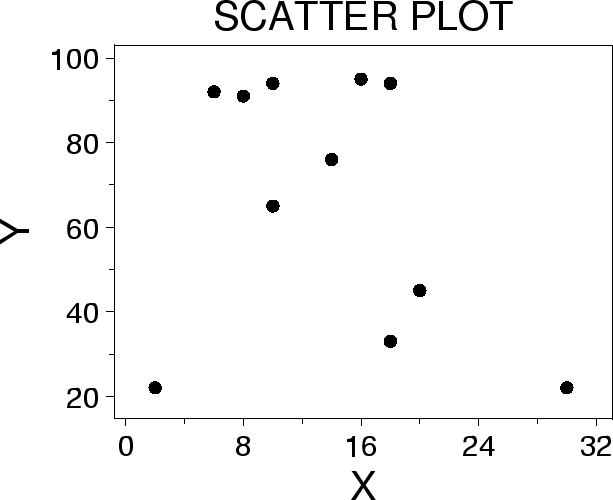
\includegraphics[width=4cm, height=3cm]{scatter-plot.png} 
\end{center}\begin{itemize}
\item In a scatter plot, the data is displayed as a collection of points.\pause
\item Each point determines it's position on the x and y axes. 
\end{itemize}
\end{frame}
%%%%%%%%%%%%%%%%%%%%%%%%%%%%%%%%%%%%%%%%%%%%%%%%%%%%%%%%%%%%%%%%%%%%%%%%%%%%%%%%
\begin{frame}
\frametitle{Exercise 1}
Plot a scatter plot showing the percentage profit of Company A from the year 2000
to 2010. The data for the same is available in the file `company-a-data.txt'.
\end{frame}
\begin{frame}[fragile]
\frametitle{scatter() function}
scatter() function is used to generate the scatter graph \pause

\begin{itemize}
\item \emph{Syntax :} \texttt{scatter(x,y)}\pause
\begin{itemize}
\item x - a sequence of data\pause
\item y - a sequence of data, the same length of x
\end{itemize}
\end{itemize}
\end{frame}
%%%%%%%%%%%%%%%%%%%%%%%%%%%%%%%%%%%%%%%%%%%%%%%%%%%%%%%%%%%%%%%%%%%%%%%%%%%%%%%%
\begin{frame}[fragile]
\frametitle{Exercise 2}
\begin{itemize}
\item Read the documentation of scatter and plot a scatter plot of the same data in `company-a-data.txt' with red diamond markers.
\end{itemize}
\end{frame}
%%%%%%%%%%%%%%%%%%%%%%%%%%%%%%%%%%%%%%%%%%%%%%%%%%%%%%%%%%%%%%%%%%%%%%%%%%%%%%%%
\begin{frame}
\frametitle{Log-log graph}
\label{sec-16}
\begin{itemize}
\item Log-log graph is
\begin{itemize}
\item two-dimensional graph of numerical data.\pause
\item it uses logarithmic scales on both axes.\pause
\item graph appears as straight line due to non-linear scaling.
\end{itemize}
\end{itemize}
\end{frame}

%%%%%%%%%%%%%%%%%%%%%%%%%%%%%%%%%%%%%%%%%%%%%%%%%%%%%%%%%%%%%%%%%%%%%%%%%%%%%%%%
\begin{frame}[fragile]
\frametitle{loglog()function}
\label{sec-18}
\begin{itemize}
\item Syntax : \texttt{loglog(x, y)}\pause
\begin{itemize}
\item \texttt{x} - a sequence of data\pause
\item \texttt{y} - a sequence of data, the same length of \texttt{x}
\end{itemize}
\end{itemize}
\end{frame}
%%%%%%%%%%%%%%%%%%%%%%%%%%%%%%%%%%%%%%%%%%%%%%%%%%%%%%%%%%%%%%%%%%%%%%%%%%%%%%%%
\begin{frame}
\frametitle{Exercise 3}
Plot a log-log chart of $y = 5x^3$ for $x$ from 1-20.
\end{frame}
%%%%%%%%%%%%%%%%%%%%%%%%%%%%%%%%%%%%%%%%%%%%%%%%%%%%%%%%%%%%%%%%%%%%%%%%%%%%%%%%
\begin{frame}
\frametitle{Summary}
\label{sec-20}
In this tutorial, we learnt to -\pause
\begin{itemize}
\item Plot a scatter plot using \texttt{scatter()} function\pause
\item Plot a log-log graph using \texttt{loglog()} function
\end{itemize}
\end{frame}
%%%%%%%%%%%%%%%%%%%%%%%%%%%%%%%%%%%%%%%%%%%%%%%%%%%%%%%%%%%%%%%%%%%%%%%%%%%%%%%%
\begin{frame}
\frametitle{Evaluation}
\begin{enumerate}
\item \texttt{scatter(x, y, color='blue', marker='d')} 
and \\
\texttt{plot(x, y,color='b', marker='d')} does exactly the same.
\begin{itemize}
	\item True
	\item False
\end{itemize}
\seti
\end{enumerate}
\end{frame}
%%%%%%%%%%%%%%%%%%%%%%%%%%%%%%%%%%%%%%%%%%%%%%%%%%%%%%%%%%%%%%%%%%%%%%%%%%%%%%%%
\begin{frame}
\frametitle{Solutions}
\label{sec-22}
\begin{enumerate}
\item False\pause
\end{enumerate}
\end{frame}
%%%%%%%%%%%%%%%%%%%%%%%%%%%%%%%%%%%%%%%%%%%%%%%%%%%%%%%%%%%%%%%%%%%%%%%%%%%%%%%%
\begin{frame}
\frametitle{Forum to answer questions}
\begin{itemize}
\item Do you have questions in THIS Spoken Tutorial?
\item Choose the minute and second where you have the question.
\item Explain your question briefly.
\item Someone from the FOSSEE team will answer them. Please visit 
\end{itemize}
\begin{center}
{\color{blue}{http://forums.spoken-tutorial.org/}}
 \end{center} 
\end{frame}
%%%%%%%%%%%%%%%%%%%%%%%%%%%%%%%%%%%%%%%%%%%%%%%%%%%%%%%%%%%%%%%%%%%%%%%%%%%%%%%%
\begin{frame}
\frametitle{Forum to answer questions}
\begin{itemize}
\item Questions not related to the Spoken Tutorial?
\item Do you have general / technical questions on the Software?
\item Please visit the FOSSEE Forum
\begin{center}
{\color{blue}{http://forums.fossee.in/}}
 \end{center}
\item Choose the Software and post your question.
\end{itemize}
\end{frame}
%%%%%%%%%%%%%%%%%%%%%%%%%%%%%%%%%%%%%%%%%%%%%%%%%%%%%%%%%%%%%%%%%%%%%%%%%%%%%%%%
\begin{frame}
\frametitle{Textbook Companion Project}
\begin{itemize}
\item The FOSSEE team coordinates coding of solved examples of popular
  books 
\item We give honorarium and certificate to those who do this
\end{itemize}
For more details, please visit this site:
\begin{center}
{\color{blue}{http://tbc-python.fossee.in/}}
\end{center}
\end{frame}
%%%%%%%%%%%%%%%%%%%%%%%%%%%%%%%%%%%%%%%%%%%%%%%%%%%%%%%%%%%%%%%%%%%%%%%%%%%%%%%%
\begin{frame}
\frametitle{Acknowledgements}
\begin{itemize}
\item Spoken Tutorial Project is a part of the Talk to a Teacher  project 
\item It is supported by the National Mission on Education through  ICT, MHRD, Government of India 
\item More information on this Mission is available at: \\{\color{blue}\url{http://spoken-tutorial.org/NMEICT-Intro}}
\end{itemize}
\end{frame}
%%%%%%%%%%%%%%%%%%%%%%%%%%%%%%%%%%%%%%%%%%%%%%%%%%%%%%%%%%%%%%%%%%%%%%%%%%%%%%%%
\begin{frame}

  \begin{block}{}
  \begin{center}
  \textcolor{blue}{\Large THANK YOU!} 
  \end{center}
  \end{block}
\begin{block}{}
  \begin{center}
    For more Information, visit our website\\
    {http://fossee.in/}
  \end{center}  
  \end{block}
\end{frame}

\end{document}
